%%%%%%%%%%%%%%%%%%%%%%%%%%%%%%%%%%%%%%%%%
% Beamer Presentation
% LaTeX Template
% Version 1.0 (10/11/12)
%
% This template has been downloaded from:
% http://www.LaTeXTemplates.com
%
% License:
% CC BY-NC-SA 3.0 (http://creativecommons.org/licenses/by-nc-sa/3.0/)
%
%%%%%%%%%%%%%%%%%%%%%%%%%%%%%%%%%%%%%%%%%

%--------------------------------------------------------------------------------
%	PACKAGES AND THEMES
%--------------------------------------------------------------------------------

\documentclass[unicode]{beamer}

\mode<presentation> {

% The Beamer class comes with a number of default slide themes
% which change the colors and layouts of slides. Below this is a list
% of all the themes, uncomment each in turn to see what they look like.

%\usetheme{default}
%\usetheme{AnnArbor}
%\usetheme{Antibes}
%\usetheme{Bergen}
%\usetheme{Berkeley}
%\usetheme{Berlin}
%\usetheme{Boadilla}
%\usetheme{CambridgeUS}
%\usetheme{Copenhagen}
%\usetheme{Darmstadt}
%\usetheme{Dresden}
%\usetheme{Frankfurt}
%\usetheme{Goettingen}
%\usetheme{Hannover}
%\usetheme{Ilmenau}
%\usetheme{JuanLesPins}
%\usetheme{Luebeck}
\usetheme{Madrid}
%\usetheme{Malmoe}
%\usetheme{Marburg}
%\usetheme{Montpellier}
%\usetheme{PaloAlto}
%\usetheme{Pittsburgh}
%\usetheme{Rochester}
%\usetheme{Singapore}
%\usetheme{Szeged}
%\usetheme{Warsaw}

% As well as themes, the Beamer class has a number of color themes
% for any slide theme. Uncomment each of these in turn to see how it
% changes the colors of your current slide theme.

%\usecolortheme{albatross}
%\usecolortheme{beaver}
%\usecolortheme{beetle}
%\usecolortheme{crane}
%\usecolortheme{dolphin}
%\usecolortheme{dove}
%\usecolortheme{fly}
%\usecolortheme{lily}
%\usecolortheme{orchid}
%\usecolortheme{rose}
%\usecolortheme{seagull}
%\usecolortheme{seahorse}
%\usecolortheme{whale}
%\usecolortheme{wolverine}

%\setbeamertemplate{footline} % To remove the footer line in all slides uncomment this line
%\setbeamertemplate{footline}[page number] % To replace the footer line in all slides with a simple slide count uncomment this line

%\setbeamertemplate{navigation symbols}{} % To remove the navigation symbols from the bottom of all slides uncomment this line

}

\usepackage{amsmath}
\usepackage{amssymb}
\usepackage{booktabs} % Allows the use of \toprule, \midrule and \bottomrule in tables
\usepackage{hyperref}
\usepackage{graphicx} % Allows including images
\usepackage{multirow}
\usepackage[russian]{babel}
\usepackage[utf8]{inputenc}

\setbeamertemplate{footnote}{\noindent\raggedright\insertfootnotetext\par}

%--------------------------------------------------------------------------------
%	TITLE PAGE
%--------------------------------------------------------------------------------

\title[]{Вероятностные тематические модели на основе данных о со-встречаемости слов}

\author{Михаил Солоткий}
\institute[ВМК МГУ] % Your institution as it will appear on the bottom of every slide, may be shorthand to save space
{
    Московский государственный университет им. М. В. Ломоносова \\
    Факультет вычислительной математики и кибернетики \\
    Кафедра математических методов прогнозирования \\
    \bigskip
    {\bf Выпускная квалификационная работа бакалавра} \\
    \bigskip
    Научный руководитель --- д.ф-м.н. Воронцов К. В.
    \bigskip
}
\date{Москва 2019 г.} % Date, can be changed to a custom date

\begin{document}

\begin{frame}
\titlepage % Print the title page as the first slide
\end{frame}

%--------------------------------------------------------------------------------
%	PRESENTATION SLIDES
%--------------------------------------------------------------------------------

%------------------------------------------------
\section{Постановка задачи}
%------------------------------------------------

\subsection{Тематическое моделирование, модель PLSA}
\begin{frame}
\frametitle{Тематическое моделирование, модель PLSA}
\footnotetext{Hofmann T., 1999: Probabilistic latent semantic analysis}
Тематическое моделирование --- один из подходов к статистическому анализу текстов. \newline

{\bf Дано}: коллекция текстовых документов $D$, словарь токенов $W$, счётчики вхождения токенов в документы $n_{dw}$. Каждый токен в каждом документе описывается некоторой скрытой темой $t \in T$. \newline

{\bf Найти}: вероятностные распределения $\Phi = \Prob(w | t)$, $\Theta = \Prob(t | d)$ методом максимального правдоподобия:
$$\frac{n_{dw}}{\sum_w n_{dw}} \approx \Prob(w | d) = \sum_{t \in T} \Prob(w | t) \Prob(t | d)$$

$$\mathcal{L}(\Phi, \Theta) = \sum_{d, w} n_{dw} \ln \sum_{t \in T} \phi_{wt} \theta_{td} \rightarrow \max_{\Phi, \Theta}$$
\end{frame}


\subsection{Аддитивная регуляризация тематических моделей}
\begin{frame}
\frametitle{Аддитивная регуляризация тематических моделей}
\footnotetext{Воронцов К. В. Аддитивная регуляризация тематических моделей коллекций текстовых документов.  Доклады РАН  2014}
АРТМ --- один из подходов к регуляризации log-правдоподобия:
$$\mathcal{L}(\Phi, \Theta) = \sum_{d, w} n_{dw} \ln \sum_{t \in T} \phi_{wt} \theta_{td} + \sum_{i=1}^k \tau_i R_i(\Phi, \Theta) \rightarrow \max_{\Phi, \Theta}$$
\begin{itemize}
    \item Желаемые свойства полученных тем можно формализовать в виде регуляризаторов $R_i(\Phi, \Theta)$
    \item Можно оптимизировать EM-алгоритмом
\end{itemize}
\end{frame}


\subsection{Меры качества тематических моделей}
\begin{frame}
\frametitle{Меры качества тематических моделей}
\begin{itemize}
    \item Перплексия:
    $$\mathcal{P}(D) = \exp \bigg( -\frac{1}{n} \sum_{d \in D} \sum_{w \in d} n_{wd} \ln \Prob(w|d) \bigg)$$
    \item Средняя (по темам) когерентность:
    $$ C = \frac{1}{|T|} \frac{2}{m(m-1)} \sum_{t \in T} \sum_{i=1}^{m-1} \sum_{j=i+1}^m \text{SPPMI}_k (w_{ti}, w_{tj})$$
    SPPMI (Shifted Positive Pointwise Mutual Information):
    $$ \text{PMI} (w_i, w_j) = \ln \frac{\Prob(w_i, w_j)}{\Prob(w_i) \Prob(w_j)}$$
    $$\text{SPPMI}_k = \max(0, \text{PMI}(w_i, w_j) - \ln k)$$
\end{itemize}
\end{frame}


\subsection{Обоснование PMI как меры интерпретируемости тем}
\begin{frame}
\frametitle{Обоснование PMI как меры интерпретируемости тем}
\footnotetext{Newman, D., Lau, J.H., Grieser, K., Baldwin, T., 2010: Automatic evaluation of topic coherence}
Newman et al показали, что средняя PMI хорошо коррелирует с человеческими оценками интерпретируемости. \\

\begin{table}[ht]
\scalebox{0.65}{
    \begin{tabular}{ c  c  c  c } \hline
        \bf Resource & \bf Method & \bf Median & \bf Mean \\ \hline
        \multirow{9}{*}{WordNet} & HSO & 0.15 & 0.59 \\
        & JCn & -0.2 & 0.19 \\
        & LCh & -0.31 & -0.15 \\
        & Lesk & \underline{0.53} & \underline{0.53} \\
        & Lin & 0.09 & 0.28 \\
        & Path & 0.29 & 0.12 \\
        & Res & 0.57 & 0.66 \\
        & Vector & -0.8 & 0.27 \\
        & WuP & 0.41 & 0.26 \\ \hline
        \multirow{4}{*}{Wikipedia} & RACO & 0.62 & 0.69 \\
        & MiW & 0.68 & 0.70 \\
        & DocSim & 0.59 & 0.60 \\
        & PMI & \bf \underline{0.74} & \bf \underline{0.77} \\ \hline
        \multirow{2}{*}{Google} & Titles & \multicolumn{2}{c}{\underline{0.51}} \\
        & LogHits & \multicolumn{2}{c}{-0.19} \\ \hline
        Gold-standard & IAA & 0.82 & 0.78 \\
        \hline
    \end{tabular}
}
\end{table}
\end{frame}

%------------------------------------------------
\section{Обучение модели}
%------------------------------------------------

\subsection{Обучение PLSA, рост когерентности}
\begin{frame}
\frametitle{Обучение PLSA, рост когерентности}

Обучение модели PLSA на коллекции статей журнала <<NY Times>>

\begin{center}
    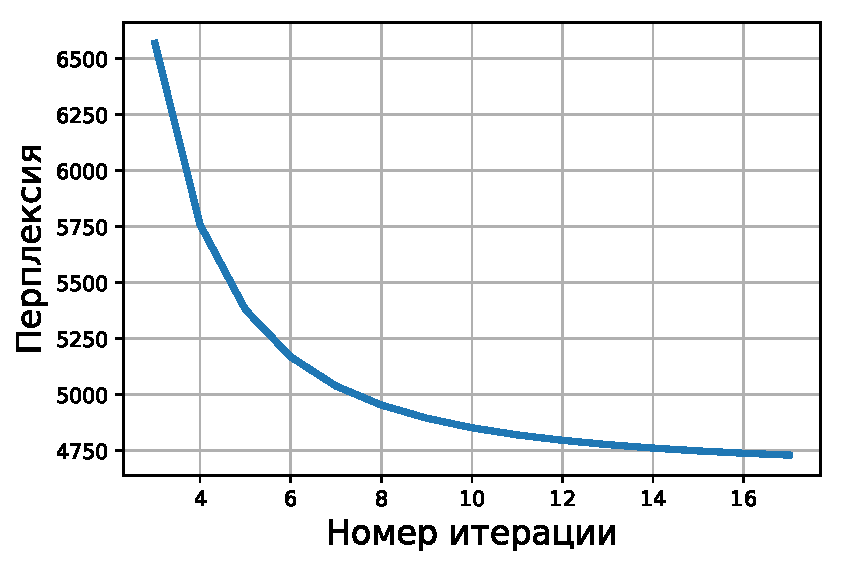
\includegraphics[scale=0.38]{perplexity_plsa_nytimes.pdf}
    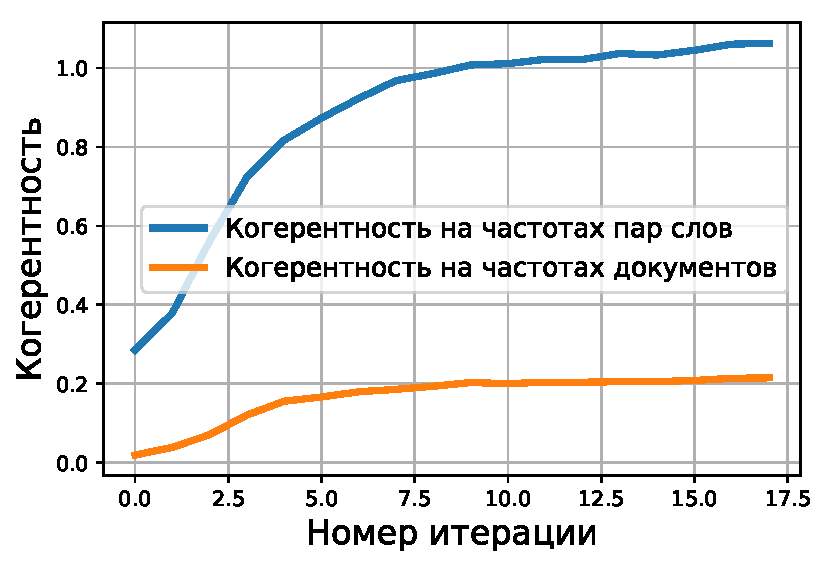
\includegraphics[scale=0.38]{coherence_plsa_nytimes.pdf}
\end{center}

\begin{itemize}
    \item Перплексия падает, она явно минимизируется
    \item Когерентность растёт, но явно она нигде в функционале не участвует
\end{itemize}
\end{frame}

%------------------------------------------------
\section{Цели и задачи}
%------------------------------------------------

\subsection{Цели и задачи}
\begin{frame}
\frametitle{Цели и задачи}
\begin{itemize}
    \item Придумать и реализовать эффективный алгоритм подсчёта статистики со-встречаемости по большим коллекциям \newline
    \item Сравнить разные статистики со-встречаемостей по качеству построенных тематических моделей \newline
    %\item Сравнить разные регуляризаторы когерентности по качеству \newline
    \item Показать, что можно без серьёзного ухудшения перплексии \newline существенно увеличивать когерентность модели
\end{itemize}
\end{frame}

%------------------------------------------------
\section{Вероятность совместной встречаемости токенов}
%------------------------------------------------

\subsection{Вероятность совместной встречаемости токенов}
\begin{frame}
\frametitle{Вероятность совместной встречаемости токенов}
Со-встречаемость пар токенов:
$$n_{uv} = \sum_{d = 1}^{|D|} \sum_{i = 1}^{n_d} \sum_{j = 1}^{n_d}
		[0 < |i - j| \leq k] [w_{di} = u] [w_{dj} = v] $$
$$n_{u} = \sum_{v \in W} n_{uv} \,\,\,\,\,\,\,
n_{v} = \sum_{u \in W} n_{uv}$$
$$n = \sum_{(u, v) \in W^2} n_{uv}$$
$$\text{PMI}(u, v) = \ln \Big[ \frac{n_{uv} n}{n_u n_v} \Big]$$    
\end{frame}


\subsection{Вероятность совместной встречаемости токенов}
\begin{frame}
\frametitle{Вероятность совместной встречаемости токенов}
Документная со-встречаемость:
$$n_{uv} = \Bigg| \Big\{ d \in D \, \big| \, \exists \, (i, j): w_{di} = u, \, w_{dj} = v, \, 0 < |i - j| \leq k \Big\} \Bigg|$$
$n_u$ --- количество документов, в которых встретился токен $u$ \\
$n_v$ --- количество документов, в которых встретился токен $v$ \\
$n$ --- количество документов всего
$$\text{PMI}(u, v) = \ln \Big[ \frac{n_{uv} n}{n_u n_v} \Big]$$    
\end{frame}

%------------------------------------------------
\section{Регуляризаторы}
%------------------------------------------------

\subsection{Регуляризатор когерентности}
\begin{frame}
\frametitle{Регуляризатор когерентности}
\footnotetext{Vorontsov, K., Potapenko, A.: Additive regularization of topic models. Machine Learning 101(1), 303–323 (2015)}
    $$R(\Phi) = -\sum_{t \in T} n_t ~\text{KL} \big( \hat{\Prob}(u | t) ~||~ \phi_{ut} \big)$$
    По формуле полной вероятности:
    $$\hat{\Prob}(u | t) = \sum_{v \in W} \Prob_{cooc}(u | v) \Prob(v | t)$$
    Формула M-шага:
    $$\phi_{wt} = \underset{w \in W}{\text{norm}} \Big( n_{wt} + \tau \sum_{v \in W \backslash w} \Prob_{cooc}(u | v) \, n_{vt} \Big)$$
\end{frame}


%\subsection{WNTM}
%\begin{frame}
%\frametitle{WNTM}
%WNTM --- это модель PLSA, построенная на псевдодокументах
%$$\Prob(w | d_u) = \sum_{t \in T} \Prob(w | t) \Prob(t | d_u) = \sum_{t \in T} \phi_{wt} \theta_{tu}$$
%Запишем как регуляризатор log-правдоподобие модели WNTM:
%$$R(\Phi, \Theta) = \sum_{(u, w) \in W^2} n_{uw} \, \ln \sum_{t \in T} \phi_{wt} \theta_{tu}$$
%Если сконкатенировать исходную коллекцию и псевдоколлекцию и будем обучать PLSA, получим:
%$$\mathcal{L}(\Phi, \Theta) = \sum_{d \in D \cup D'} \sum_{w \in W} n_{dw} \ln \sum_{t \in T} \phi_{wt} \theta_{td} =$$
%$$= \sum_{d \in D} \sum_{w \ in W} n_{dw} \ln \sum_{t \in T} \phi_{wt} \theta_{td} + R(\Phi, \Theta)$$
%\end{frame}

%------------------------------------------------
\section{Алгоритм сбора статистики со-встречаемостей}
%------------------------------------------------

\subsection{Алгоритм сбора статистики со-встречаемостей}
\begin{frame}
\frametitle{Алгоритм сбора статистики со-встречаемостей}
3 этапа:
\begin{enumerate}
    \item Обработка входной коллекции:
        \begin{itemize}
            \item Загрузка в оперативную память $batch\_size$ документов
            \item Параллельная обработка
            \item Сохранение статистики со-встречаемостей по пакетам во внешнюю память в отсортированном формате
        \end{itemize}
    \item Слияние файлов с помощью k-Way Merge
    \begin{itemize}
        \item Если файлов слишком много, многошаговое слияние
    \end{itemize}
    \item Вычисление PMI
\end{enumerate}

Реализован в библиотеке тематического моделирования BigARTM
\footnotetext{https://github.com/bigartm/bigartm} \newline \newline
Время работы: $\mathcal{O} \big( |D| +  |W|^2 \big)$ \\
Оперативная память: $\mathcal{O} \big( 1 \big)$ \\
Внешняя память: $\mathcal{O} \big( |D| \log |D| \big)$
\end{frame}


\subsection{Эксперимент на корпусе Википедии}
\begin{frame}
\frametitle{Эксперимент на корпусе Википедии}
Обработка полного текста англоязычной Википедии:
\begin{itemize}
    \item $\approx$ 20 Гб текста
    \item $\approx$ 8.5 млн статей
    \item $\approx$ 8.2 млн уникальных токенов
    \item $\approx$ 3.8 млрд токенов всего
    \item $window\_width = 10$
\end{itemize}

В результате:
\begin{itemize}
    \item время работы: 4 часа 18 минут на ноутбуке с 8-ядерным процессором
    \item около 130 Гб занимают промежуточные файлы
\end{itemize}
\end{frame}

%------------------------------------------------
\section{Результаты}
%------------------------------------------------

\subsection{KL-регуляризатор, разные типы когерентности}
\begin{frame}
\frametitle{KL-регуляризатор, разные типы когерентности}

\begin{center}
    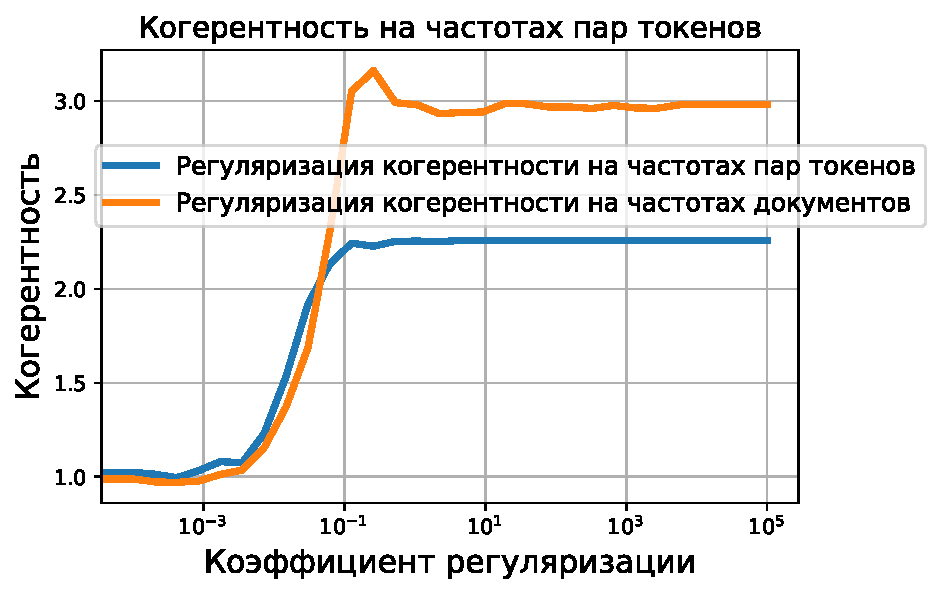
\includegraphics[scale=0.35]{coherence_tf_score_reg_on_ppmi_tf_df_nytimes.pdf}
    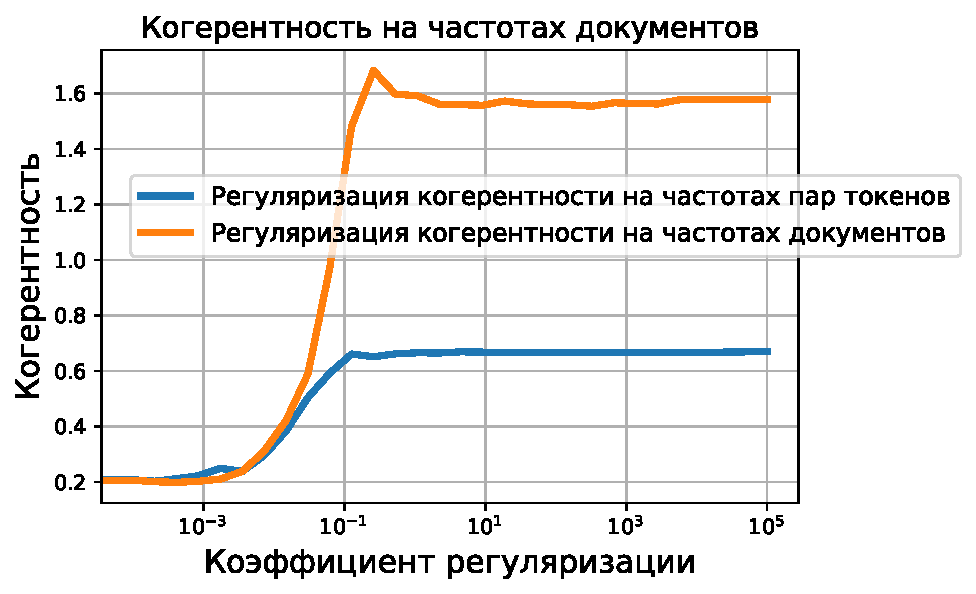
\includegraphics[scale=0.35]{coherence_df_score_reg_on_ppmi_tf_df_nytimes.pdf}
\end{center}

\begin{center}
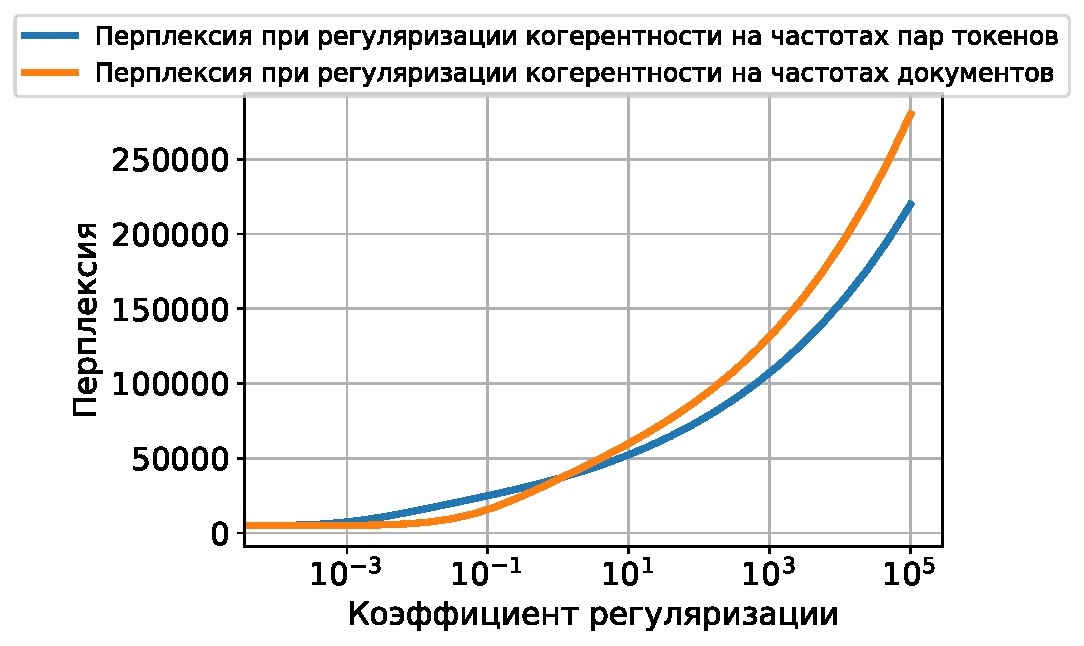
\includegraphics[scale=0.35]{perplexity_tf_df_on_ppmi_nytimes.pdf}
\end{center}
\end{frame}


\subsection{Зависимость когерентности от количества тем}
\begin{frame}
\frametitle{Зависимость когерентности от количества тем}
\begin{center}
    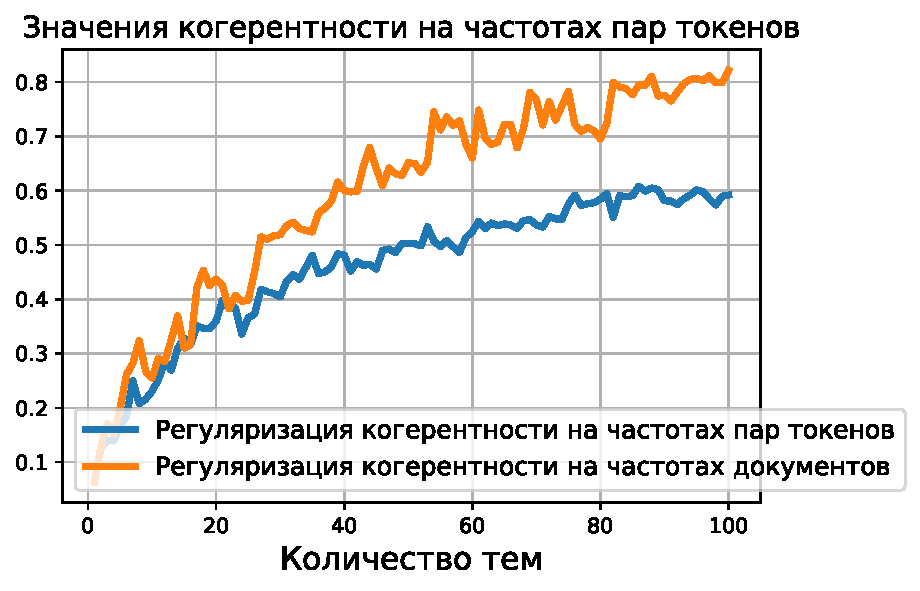
\includegraphics[scale=0.30]{coherence_tf_reg_tf_df_score_with_different_num_of_topics.pdf} \,\,\,\,\,
    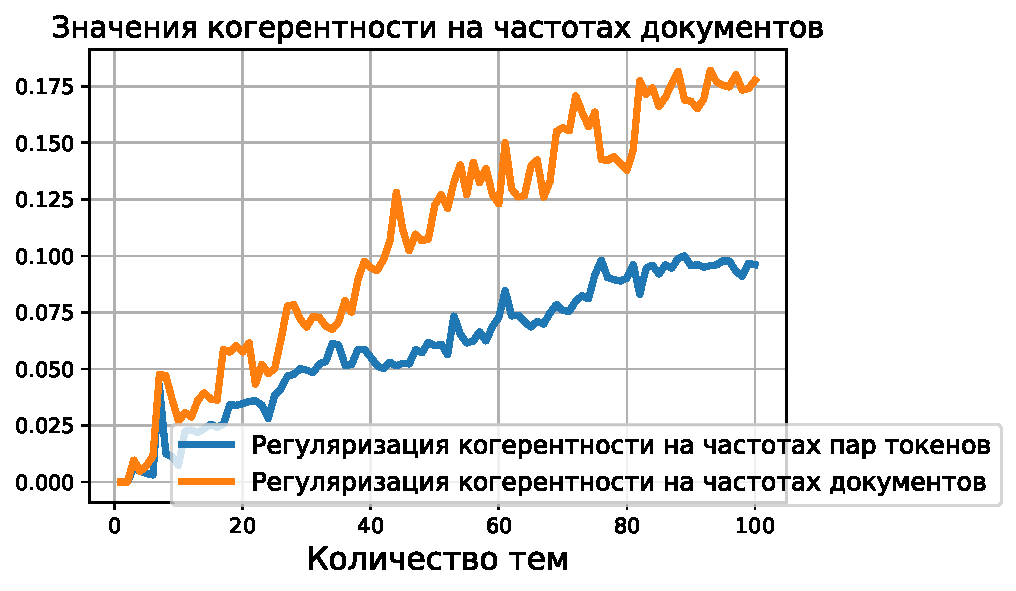
\includegraphics[scale=0.30]{coherence_df_reg_tf_df_score_with_different_num_of_topics.pdf}
\end{center}
\begin{center}
    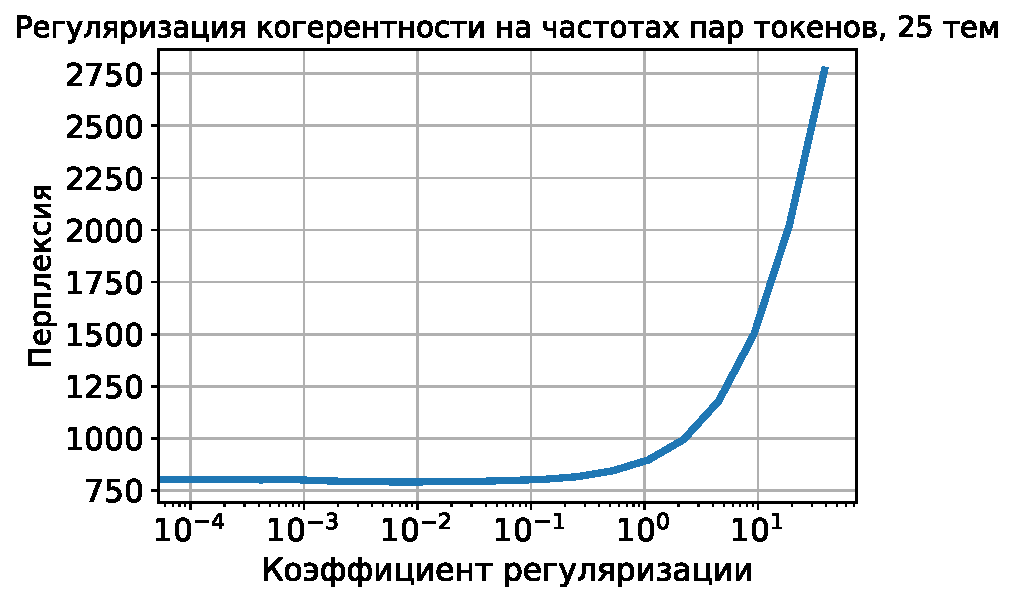
\includegraphics[scale=0.30]{perplexity_coherence_tf_reg_25_topics.pdf}
    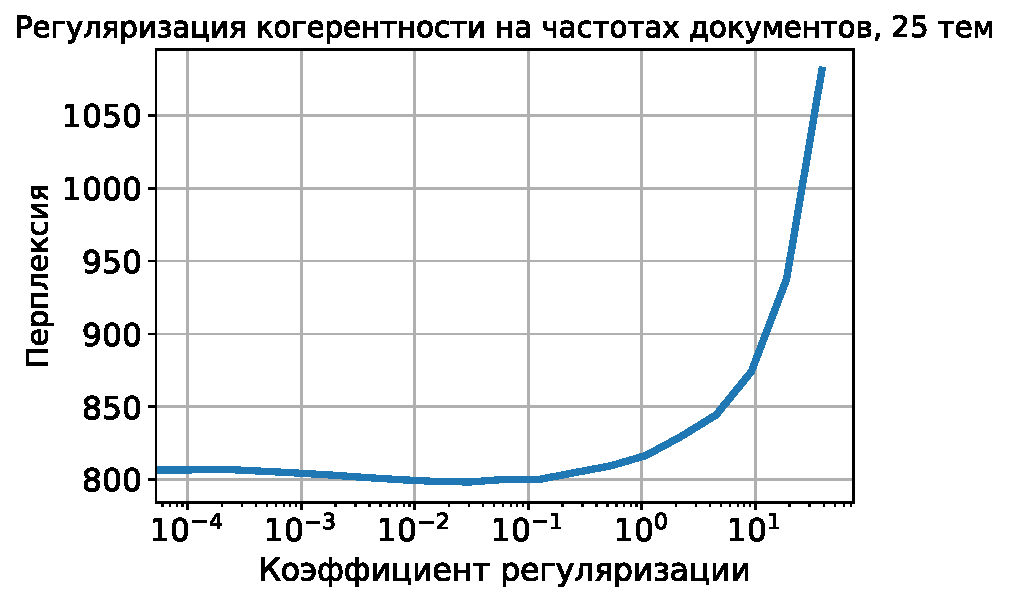
\includegraphics[scale=0.30]{perplexity_coherence_df_reg_25_topics.pdf}
\end{center}
\end{frame}


\subsection{Эксперимент регуляризацией когерентности}
\begin{frame}
\frametitle{Эксперимент с регуляризацией когерентности}
\begin{enumerate}
    \item Регуляризация когерентности на частотах документов
    \item Экспоненциальное уменьшение коэффициента регуляризации
    \item Достаточно большое число тем
\end{enumerate}
\begin{center}
    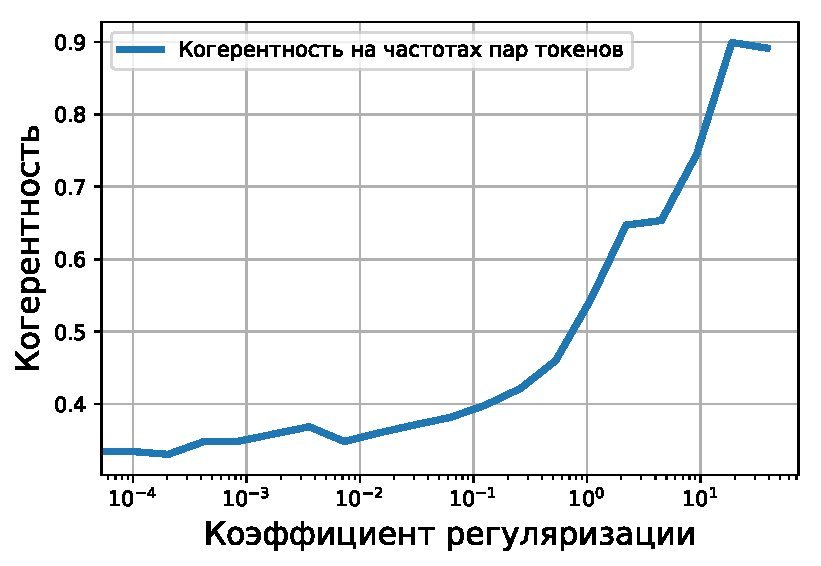
\includegraphics[scale=0.30]{coherence_df_reg_on_ppmi_mmro_tf_score.pdf}
    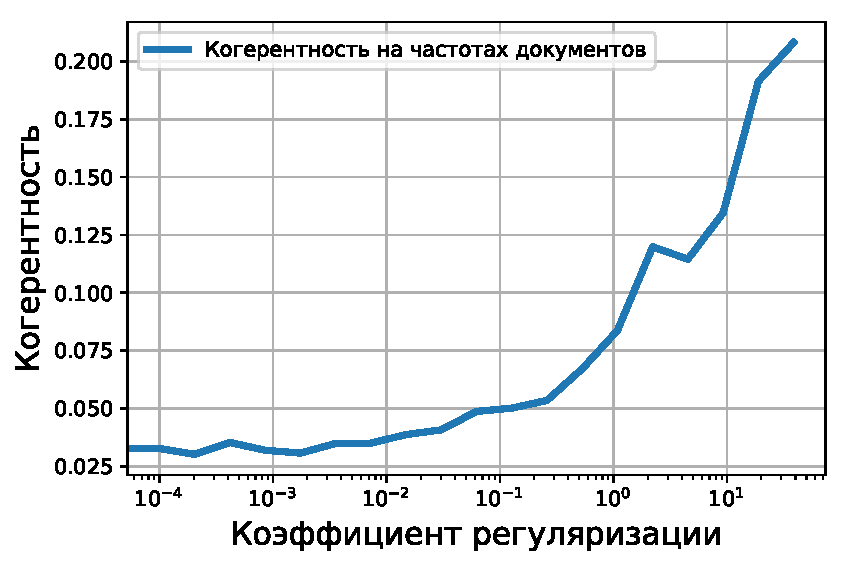
\includegraphics[scale=0.30]{coherence_df_reg_on_ppmi_mmro_df_score.pdf}
    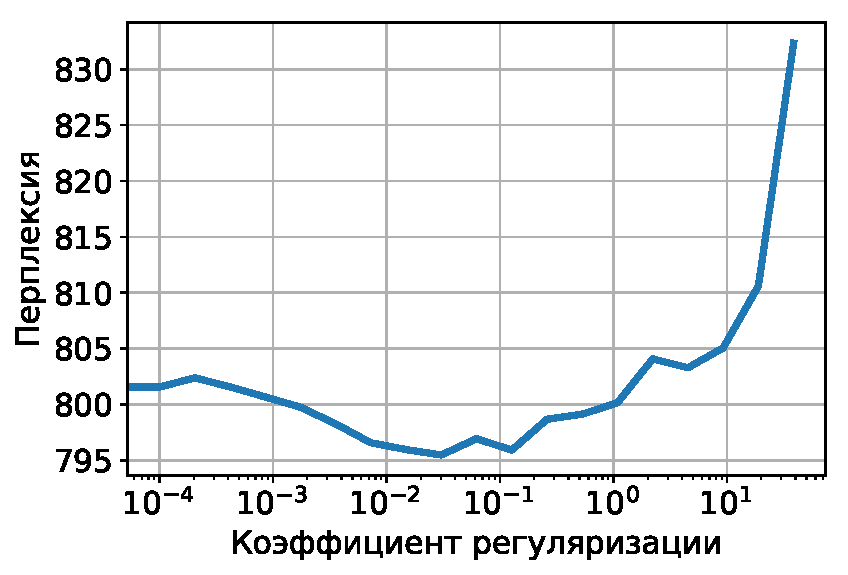
\includegraphics[scale=0.30]{perplexity_tf_reg_on_ppmi_mmro.pdf}
    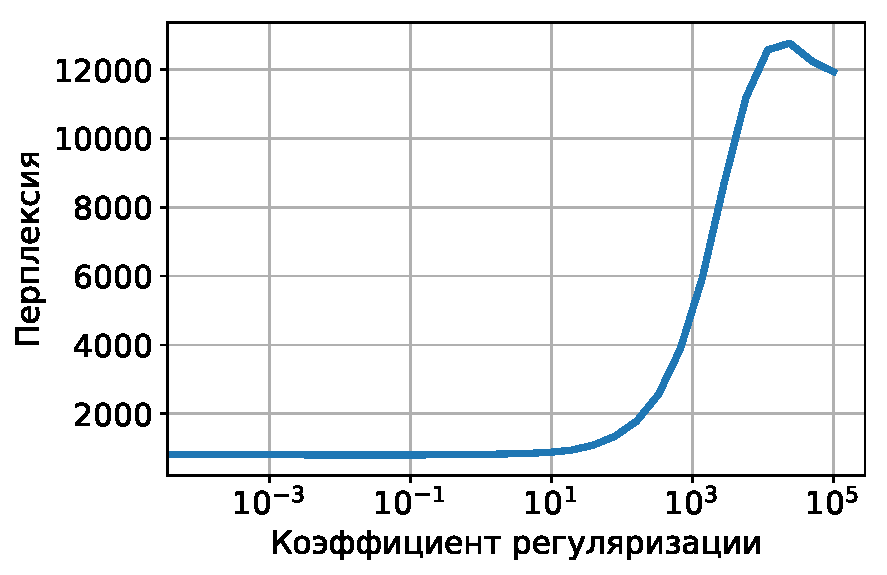
\includegraphics[scale=0.30]{perplexity_df_reg_on_ppmi_mmro_full.pdf}
\end{center}
\end{frame}


\subsection{Возможные применение данных со-встречаемости в ВТМ}
\begin{frame}

\frametitle{Возможные применение данных со-встречаемости в ВТМ}
\begin{itemize}
    \item Измерение когерентности тематической модели \newline
    \item Регуляризаторы когерентности \newline
    \item Модель битермов BitermTM \newline
    \item Модель WNTM (Word Network Topic Model)
\end{itemize}

\footnotetext{
    \emph{Xiaohui Yan, Jiafeng Guo, Yanyan Lan, Xueqi Cheng}.
    A~Biterm Topic Model for Short Texts. WWW 2013.
}
\footnotetext{
    \emph{Yuan Zuo, Jichang Zhao, Ke Xu.}
    Word Network Topic Model: a simple but general solution for short and imbalanced texts. 2014.
}
\footnotetext{
    \emph{A.Potapenko, A.Popov, K.Vorontsov.}
    Interpretable probabilistic embeddings: bridging the gap between topic models and neural networks. AINL-6, 2017.
}
\end{frame}

\subsection{Результаты, выносимые на защиту}
\begin{frame}
\frametitle{Результаты, выносимые на защиту}
\begin{itemize}
    \item Предложен метод повышения когерентности тематических моделей и исследованы условия его применимости \newline
    \item Предложен и реализован эффективный параллельный пакетный алгоритм для вычисления статистики совместной встречаемости токенов в больших текстовых коллекциях
\end{itemize}
\end{frame}

\end{document}
